\chapter{Hybrid Traversal Selection for Efficient Source Code Analysis}
\label{sec:approach}
\label{sec:overview}
 
In this section we first provide a brief overview of our technique, 
followed by an overview of the constructs used for expressing source code analyses.
We then describe properties, analyses, and a decision tree that are 
the technical underpinnings of our selection technique.

\begin{figure*}[ht!]
  \centering 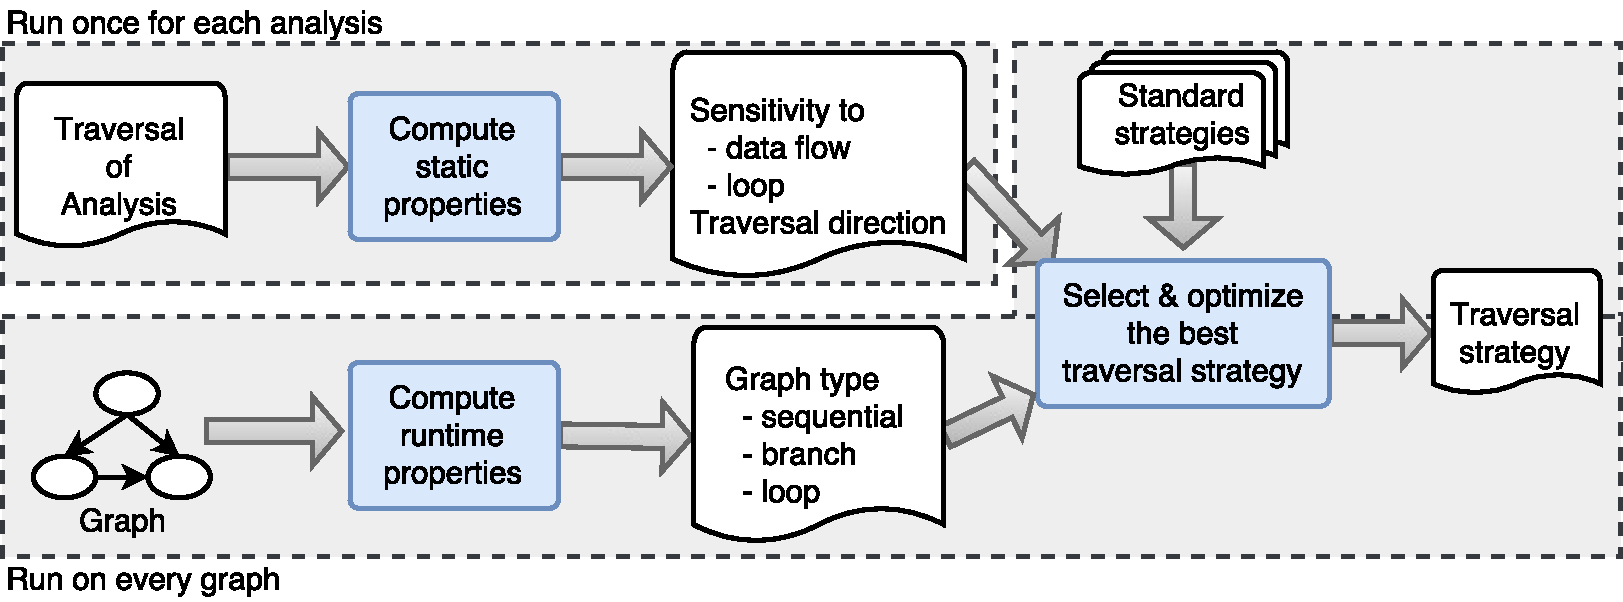
\includegraphics[width=0.9\linewidth]{figures/hybrid-overview.pdf}
\caption{Overview of the hybrid approach for selecting and optimizing graph traversal strategy.}
  \label{fig:overview}
\end{figure*}

\fignref{fig:overview} provides an overview of our approach and its key components.
Inputs to our approach are source code analysis that contains one or more 
traversals (\secref{sec:language}), and a graph. 
Output of our technique is an optimal traversal strategy for every
traversal in the analysis. For selecting an optimal traversal strategy for a
traversal, our technique computes a set of static properties of 
the analysis (\secref{sec:compute-properties}),
such as data-flow sensitivity, loop sensitivity, and extracts a runtime property
about the graph that defines the \graphprop{} in the graph
(sequential/branch/loop). Upon computing the static and runtime properties, our
approach selects a traversal strategy from a set of candidate strategies (\secref{sec:candidates}) for
each traversal in the analysis (\secref{sec:decision-tree}) and 
optimizes it (\secref{subsec:optimizations}). The static properties of the
traversals are computed only once for each analysis, whereas graph \graphprop{} 
is determined for every input graph.

\section{A System For Expressing Source Code Analysis As Traversals}
\label{sec:language}
% \section{Program analysis and traversals}
% \label{sec:programanalysis}
A source code analysis is performed on various source code artifacts such as
source code text, intermediate representations like abstract syntax trees
(ASTs), graph-based representations like control flow graphs (CFGs) and call
graphs (CGs), etc. In our system, source code analysis such as control- and
data-flow analysis are expressed as traversals over CFGs.

\begin{definition}\label{def:cfg}
A control flow graph (CFG) is a directed graph $G$ = $(N, E, n_{start},
N_{end})$ with a set of nodes $N$ representing the program statements and a set
of edges $ E \subseteq N \times N$ representing the control flow relation
between the program statements. A CFG has a single start node, $n_{start}$, and
a set of end nodes, $N_{end}$.
\end{definition}

% A source code analysis such as control flow analysis, data-flow analysis, etc can be
% expressed as traversals over program graphs.
% \begin{definition}\label{def:cfg}
% A \textbf{Program Graph} of a program is defined as $G$ = $(N, E, n_{start},
% N_{end})$, where $G$ is a directed graph with a set of nodes $N$ representing program statements,
% and a set of edges $ E \subseteq N \times N$ representing analysis relevant
% relationship between the nodes in the graph.
% 
% representing possible flow of execution between the nodes in the
% graph.
% A program graph has a single start, $n_{start}$, and a set of end nodes, 
% $N_{end}$.
% All the nodes in a program graph are reachable from the $n_{start}$ and the
% $n_{end}$ node is reachable from all nodes in the program graph.
% \end{definition}
For any node $n \in N$, $n.preds$ is a set of immediate predecessors, $n.succs$
is a set of immediate successors, $n.stmt$ provides the program statement at the
node, and $n.id$ is a unique identifier of the node. Here on, we use graph to
refer to CFG.
% Note that, depending on the analysis, node ids are assigned while constructing
% the graph. For instance, in case of control flow graphs, node ids may be
% assigned in the order of the flow of execution.
% Note that, node ids are assigned in the order of the flow of
% execution, while constructing a graph. 
% Examples of program graph includes control flow graph (CFG), control dependence
% graph (CDG), program dependence graph (PDG), etc. Hereon, we refer to program
% graphs simply as graphs. 
% 
% \newline \tab $n.preds = P$ where $P =
% \{p_{0}, p_{1},.., p_{p}\}$ such that $\forall p_{i}, (p_{i}, n) \in E$,
% \newline \tab $n.succs = S$ where $S = \{s_{0}, s_{1},.., s_{s}\}$ such that
% $\forall s_{i}, (n, s_{i}) \in E$, \newline \tab $n.stmt$ = program statement
% contained in the node $n$, \newline \tab $n.id$ = unique identifier of the node
% $n$. $ids$ are integers that are assigned to the nodes in topological order.
% \end{definition}

A source code analysis over a graph visits nodes in the graph in certain order
and collects information at nodes (aka, analysis facts or outputs). For
instance, the {\em reaching definition} analysis over a CFG, visits every node
in the CFG and collects the variable definitions at nodes as analysis facts.
An analysis may require multiple traversals over a graph and each traversal may
visit nodes multiple times (for fixpoint).
For instance, the {\em reaching definition} analysis requires two traversal of
the CFG: an {\em initialization} traversal for collecting the variable
definitions at nodes as analysis facts, and a {\em propagation} traversal for
propagating the analysis facts along the graph. The {\em initialization}
traversal visits every node exactly once, whereas the {\em propagation}
traversal may visit the nodes multiple times until a fixpoint is reached and the
analysis facts at nodes does not change further.

% A program analysis, such as control or data flow analysis visits nodes in
% the CFG, in certain order, and collects analysis facts at nodes. For
% instance, the {\em reaching definition} analysis visits every node in the CFG
% and collects variable definitions at nodes as analysis facts. An analysis
% may require multiple traversals of a CFG. For instance, the {\em reaching
% definition} analysis, in the {\em initialization} traversal, collects variable
% definitions at nodes as analysis facts, and in the {\em propagation}
% traversal, updates the analysis facts until a fixpoint is reached, where no
% further changes to analysis facts at nodes is required.

In our system, a source code analysis over a graph is expressed by defining and
invoking one or more traversals. A traversal is defined using a special
\lstinline|traversal| block: 
\begin{lstlisting} 
t := traversal(n : Node) : T { tbody }
\end{lstlisting}
In this traversal block definition, \lstinline|t| is the name of the traversal
that takes a single parameter \lstinline|n| representing the graph node that is
being visited. A traversal may define a return type \lstinline|T| representing
the output type. The output type can be a primitive or a collection data type. A
block of code that generates the traversal output at a graph node is given by
\lstinline|tbody|. The \lstinline|tbody| may contain common statements and
expressions, such as variable declarations, assignments, conditional statements,
loop statements, and method calls, along with some special expressions discussed
in this chapter.
% 
% 
% A traversal visits every node in the control flow graph and executes a block of
% code. The traversal visits the nodes in a certain fashion and produces a output
% of certain type for each node. Signature to express our traversals is shown
% below.
%\begin{verbatim}
	%t := traversal(n : Node) : OType { tbody }
%\end{verbatim}
% 
% The traversal block shown above defines a variable \lstinline|t| of
% traversal type and the traversal visits every node in the graph in certain order
% and while visiting a node \lstinline|n|, it executes a block of code
% \lstinline|tbody| to produce an output of type \lstinline|T| for the
% visited node.
% 
% A \lstinline|traversal| block always take one parameter of type \lstinline|Node|
% representing a graph node, and it has an optional output type,
% \lstinline|T|.
% The output type can be a primitive or a collection data type. 
% Semantically, a traversal that defines \lstinline|T|, generates and collects
% analysis facts for nodes in the graph.
% A block of code that generates the analysis facts at a graph node is given by
% \lstinline|tbody|. The instructions or operations in the \lstinline|tbody| block
% is defined in the language for expressing the source code analysis. A traversal
% block can be assigned a name, \lstinline|t| in the above listing, which
% can be used to invoke the traversal. The type of \lstinline|t| is a
% special traversal type. 

A traversal can be invoked using a special \lstinline|traverse| expression:
\begin{lstlisting}
traverse(g, t, d, df, ls, fp)
\end{lstlisting}

A \lstinline|traverse| expression takes six parameters: \lstinline|g| is the
graph to be traversed, \lstinline|t| is the traversal to be invoked,
\lstinline|d| is the traversal direction and \lstinline|df|, \lstinline|ls|, \lstinline|fp| are optional
parameters. \lstinline|df| is of boolean type which indicates whether the analysis is data flow sensitive or not. \lstinline|ls| is also an boolean variable, indicating whether the analysis is loop sensitive or not. If \lstinline|df| is not provided, Algorithm 1 in Chapter 3.2.1 will be used to compute this property. Similarly, if \lstinline|ls| is not provided, Algorithm 2 in Chapter 3.2.3 will be used to compute this property. \lstinline|fp| is a variable name of the user defined fixpoint function. A
traversal direction is a value from the set \{\lstinline|FORWARD|,
\lstinline|BACKWARD|, \lstinline|ITERATIVE|\}, where \lstinline|FORWARD| is used
to represent a forward analysis (predecessors of a node are processed before the
node), \lstinline|BACKWARD| is used to represent a backward analysis (successors
of a node are processed before the node), and \lstinline|ITERATIVE| is used to
represent a sequential analysis (visits nodes as they appear in the nodes
collection).
A user defined fixpoint function can be defined using the \lstinline|fixp|
block:
\begin{lstlisting}
fp := fixp(...) : bool { fbody }
\end{lstlisting}

In this \lstinline|fixp| block, \lstinline|fixp| is a keyword for defining a
fixpoint function. A fixpoint function can take any number of parameters, and it
must always return a boolean. The body of the fixpoint function is defined in
the \lstinline|fbody| block. A fixpoint function can be assigned a name, which
can be passed in the \lstinline|traverse| expression.

\para{Accessing Facts of Other Nodes}
We also provide a special expression \lstinline|output(n, t)| for querying the
traversal output associated with a graph node \lstinline|n|, in the traversal
\lstinline|t|.

\begin{table*}[ht!] \centering \small
\caption{Syntax reference.}
\label{tab:syntax}
% \resizebox{\textwidth}{!}{
\begin{tabular}{|p{1.5cm}|p{2.5cm}|p{11cm}|}
\hline 
\textbf{Construct} & \textbf{Syntax} & \textbf{Description}\\\hline
Traversal & \lstinline|t := traversal(n : Node) : T { tbody }| & \lstinline|t| is the name of the traversal that takes a single parameter \lstinline|n| representing the graph node that is being visited. A traversal may define a return type \lstinline|T| representing the output type. A block of code that generates the traversal output at a graph node is given by \lstinline|tbody|.\\\hline
Traverse & \lstinline|traverse(g, t, d, df, ls, fp)| & \lstinline|g| is the
graph to be traversed, \lstinline|t| is the traversal to be invoked,
\lstinline|d| is the traversal direction and \lstinline|df|, \lstinline|ls|, \lstinline|fp| are optional
parameters. \lstinline|df| is of boolean type which indicates whether the analysis is data flow sensitive or not. \lstinline|ls| is also an boolean variable, indicating whether the analysis is loop sensitive or not. \lstinline|fp| is a variable name of the user defined fixpoint function. A traversal direction is a value from the set \{\lstinline|FORWARD|,
\lstinline|BACKWARD|, \lstinline|ITERATIVE|\}\\\hline 
Fixpoint & \lstinline|fp := fixp(...) : bool { fbody }| & \lstinline|fixp| is a keyword for defining a fixpoint function. A fixpoint function can take any number of parameters, and it
must always return a boolean. The body of the fixpoint function is defined in
the \lstinline|fbody| block.\\\hline 
Output & \lstinline|output(n, t)| & \lstinline|output| is used for querying the
traversal output associated with a graph node \lstinline|n|, in the traversal
\lstinline|t|\\\hline 
\end{tabular}
% }
\end{table*}

% 
% 
% 
% \lstinline|tbody| represents the block of code that will be executed when
% traversing a node. Here \texttt{t} is the name of the traversal.
% The traversal \texttt{t} produces a output of OType for each visited node. This
% output can be queried by a special function \textit{output} which takes the form
% given below.
% \begin{verbatim}
% 			output(n, t)
% \end{verbatim}
% Here \texttt{n} represents the node and \texttt{t} represents the traversal.
% \textit{output} returns the output associated with the node n visited in the
% traversal t. In-order to invoke a traversal on a control flow graph, we use the
% \textit{traverse} operation.
% \begin{verbatim}
% 			traverse(g, t, d, fp); 
% \end{verbatim}
% The \textit{traverse} operation takes four arguments. where \texttt{g} is the
% control flow graph to be traversed, \texttt{t} is the traversal, \texttt{d} is
% the traversal direction which can take either of the two values
% \{\texttt{FORWARD}, \texttt{BACKWARD}\}, \texttt{fp} is the optional user
% defined fixpoint function, which will run the traversal until the fixpoint
% condition is satisified by all the nodes. Fixpoint function has the following
% syntax.
% \begin{lstlisting}[caption={Fixpoint construct.},label={lst:fixp}]
% fp := fixp(...) : bool {
%         fbody
% }
% \end{lstlisting}
% Here \textit{fixp} is a keyword and it can take any number of parameters and
% always returns a boolean. \texttt{fp} is the name of the fixpoint fucntion and
% \texttt{fbody} is the user written block of code. If the return value is
% \texttt{TRUE}, then it indicates that the fixpoint is reached. \newline There is
% no option to specify the traversal strategy in traverse operation as the best
% traversal strategy will be decided based on the input control flow graph and the
% body of the traversal. \newline

\begin{table*}[ht!] \centering \small
\caption{Operations on collections.}
\label{tab:operations}
% \resizebox{\textwidth}{!}{
\begin{tabular}{|l|l|}
\hline 
\textbf{Operation} & \textbf{Description}\\\hline
\lstinline|add(C, e)| & Adding an element e to collection C \\\hline
\lstinline|addAll(C1, C2)| & Adding all elements from collection C2 to collection
C1\\\hline 
\lstinline|remove(C, e)| & Removing an element e from collection C \\\hline 
\lstinline|removeAll(C1, C2)| & Removing all elements from collection C1 that are
also present in collection C2\\\hline 
\lstinline|get(C, i)| & Element at index i from collection C is accessed\\\hline
\lstinline|has(C, e)| & Checking if collection C has element e\\\hline
\lstinline|equals(C1, C2)| & Checking if collection C1 and collection C2 has the
same elements\\\hline 
\lstinline|C1 = C2| & Assigning collection C2 to collection C1\\\hline
\lstinline|union(C1, C2)| & Returns the union of the elements in collection C1 and
collection C2\\\hline 
\lstinline|intersection(C1, C2)| & Returns the intersection of the elements in collection C1 and collection C2\\\hline
\end{tabular}
% }
\end{table*}
\para{Data Types and Collections}
% \label{sec:Data-Types}
Our system for expressing source code analysis as traversals provides primitive and
collection data types. Primitive types include: \lstinline|bool, int, string|
and collection types include: \lstinline|Set and Seq|, where \lstinline|Set| is a
collection with distinct and unordered elements, whereas, \lstinline|Seq| is a
collection with distinct and ordered elements. A set of operations that can be
performed on collection types is described in \tabref{tab:operations}.
% 
% There are three primitive types (bool , int , string) that could be used in our
% traversal. We also provides two types of collection : Set and Sequence. Elements
% in a Set are unique but unordered. Elements in a Sequence are not unique but
% ordered. Operations that are allowed in the collection are specified in Table
% \ref{tab:operations}.

To summarize, we described a system for expressing source code analysis as
traversals over graphs using two special constructs: \lstinline|traversal| for
defining a traversal, and \lstinline|traverse| for invoking a defined traversal. 
A traversal may visit graph nodes multiple times (in case of fixpoint) and it
can be invoked using several parameters specifying the direction of the
traversal, a user defined fixpoint function, etc.
A traversal output associated with graph nodes can be queried using a special
expression \lstinline|output()|. 
To be able to express a variety of source code analysis, our system provides
primitive and collection datatypes with well-defined operations.
Later in this chapter we demonstrate how the constructs and operations of the
system enables determining properties of the source code analysis expressed
in our system, such that optimal traversal strategies can be automatically
selected.

% We also provide a special expression \lstinline|output()| to query the analysis
% output of nodes and a set of operations to compose and manipulate traversal
% output of nodes. 
% The special constructs and operations defined here solves a
% challenging problem of determining certain static properties of the analyses, as
% described in \secnref{sec:compute-properties}.
\para{An Example: Post dominator analysis} We now describe how to use our system
to express source code analysis as traversals using an example source code analysis.
Post dominator analysis is a backward control flow analysis that collects node
ids of all nodes that post dominates every node in the CFG~\cite{compilers}.
This analysis can be expressed using our system as shown in Listing
\ref{lst:dominators}.

\begin{lstlisting}[basicstyle=\footnotesize\ttfamily, numbers=left, numbersep=-8pt, 
escapechar=@, caption={Post dominator analysis: an example source code analysis
expressed using our system.}, label={lst:dominators}] 
	allNodes: Set<int>;
	initT := traversal(n: Node) { 
		add(allNodes, n.id);
	}
	domT := traversal(n: Node): Set<int> { 
		Set<int> dom;
		if (output(n, domT) != null) {
			dom = output(n, domT);
		} else {
			if (node.id == exitNodeId) {
				dom = {};
			} else {
				dom = allNodes;
			}
		}
		foreach (s : n.succs) 
			dom = intersection(dom, output(s, domT)) 
		add(dom, n.id); 
		return dom; 
	} 
	fp := fixp(Set<int> curr, Set<int> prev): bool {
		if(equals(curr, prev))
			return true;
		return false;
	}
	traverse(g, initT, ITERATIVE); @\label{line:traverse}@
	traverse(g, domT, BACKWARD, fp); 				
\end{lstlisting}

Listing \ref{lst:dominators} mainly defines two traversals \textbf{\lstinline|initT|}
(lines 2-4) and \textbf{\lstinline|domT|} (lines 5-20), and invokes them using
\textbf{\lstinline|traverse|} expressions (lines 26 and 27). Line 21-25 defines a
fixpoint function using \textbf{\lstinline|fixp|} block, which is used in the
\textbf{\lstinline|traverse|} expression in line 27. Line 1 defines a variable
\textbf{\lstinline|allNodes|} of collection type \textbf{\lstinline|Set|}, where
\textbf{\lstinline|Set<int>|} defines a collection type \textbf{\lstinline|Set|} with elements of
type \textbf{\lstinline|int|}. Line 3 uses an operation \textbf{\lstinline|add|} (defined in
\tabref{tab:operations}) on collection \textbf{\lstinline|allNodes|}. The common
statements and expressions used in the language to express the analysis are not
described in our system, however all standard statements and expressions are
allowed.
For instance, \textbf{\lstinline|if-else|} statements are used in lines 7-15,
\textbf{\lstinline|foreach|} iteration is used in lines 16-17, and so on.
Lines 26 and 27 provides two flavors of invoking traversals using
\textbf{\lstinline|traverse|} expressions: one without a fixpoint and other with a
user-defined fixpoint function. A usage of special expression
\textbf{\lstinline|output(n, domT)|} can be seen in line 8. The traversal
\textbf{\lstinline|initT|} does not define any output for CFG nodes, whereas, the
traversal \textbf{\lstinline|domT|} defines an output of type \textbf{\lstinline|Set<int>|} for
every node in the CFG. For managing the analysis output of nodes,
\textbf{\lstinline|domT|} traversal maintains an internal map that contains analysis
output for every node, which can be queried using \textbf{\lstinline|output(n, domT)|}.
A pre-defined variable \textbf{\lstinline|g|} that represents the CFG is used in the
\textbf{\lstinline|traverse|} expressions in lines 26 and 27.

\begin{figure}[ht!]
\centering
% \caption{}
% % 
% % 
% % Dominator analysis performs traversal over the graph to determine the
% % dominators of each node. It has two traversals. \textit{init} traversal collects
% % all node ids. \textit{dom\_T} is called with a fixpoint and it runs till all the
% % nodes reach the fixpoint condition.}
% \label{fig:dominator}
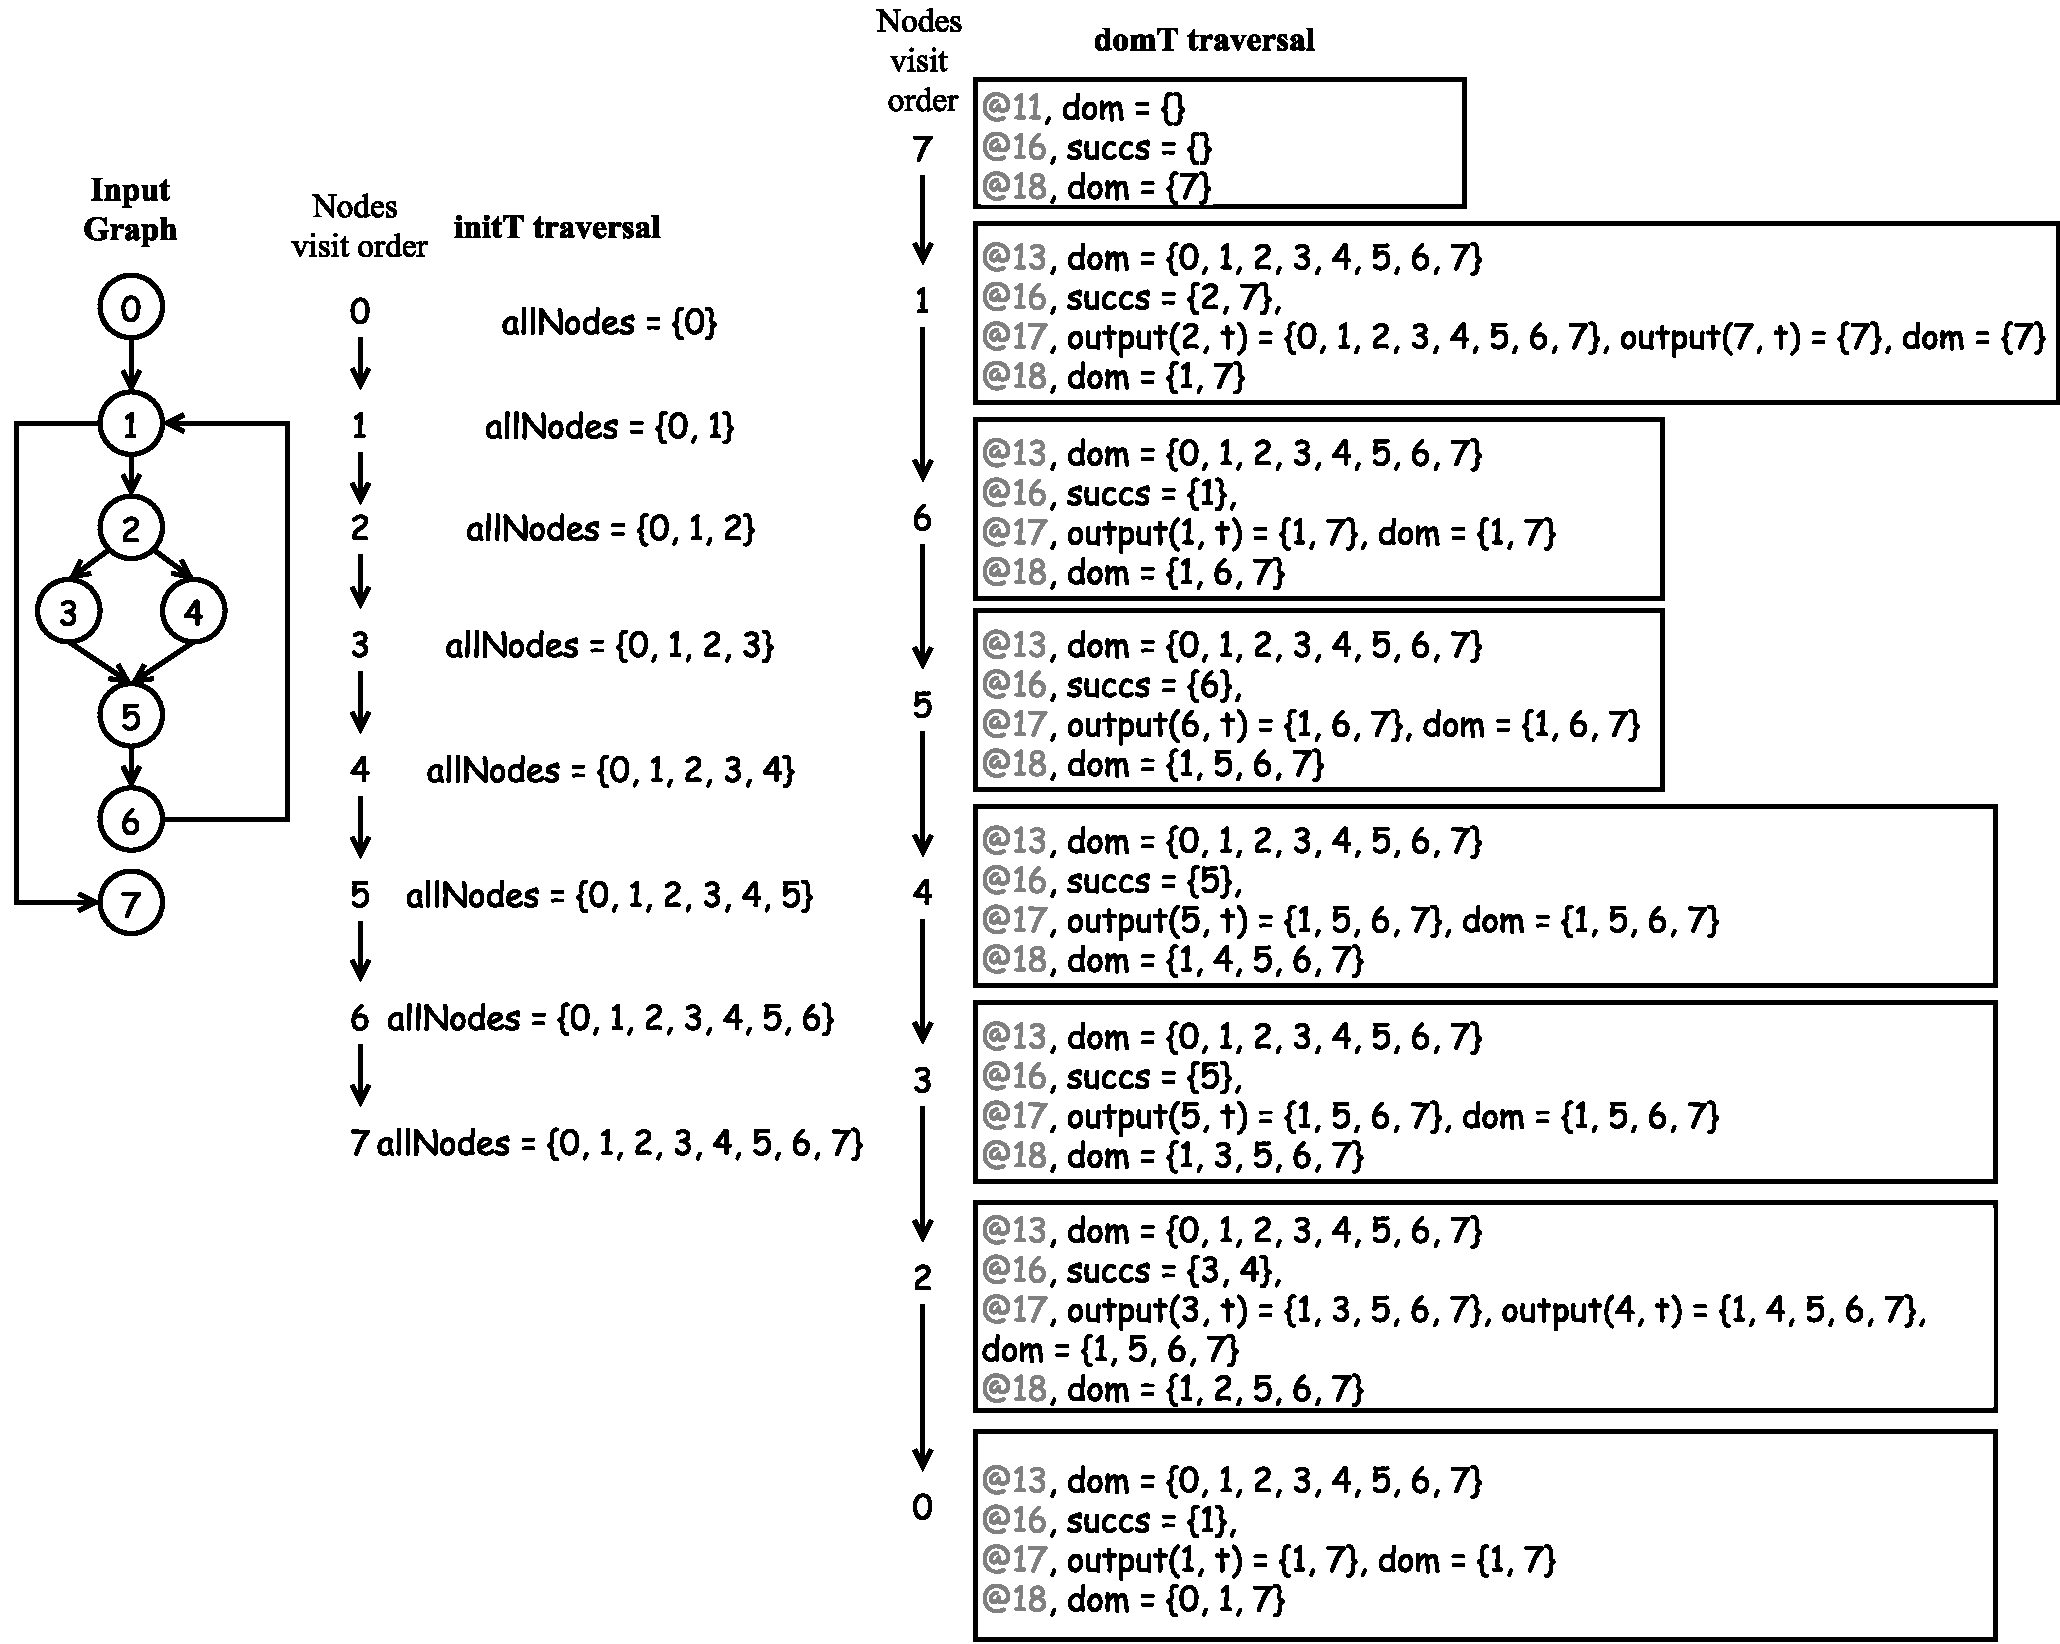
\includegraphics[width=0.9\linewidth]{figures/running-example.pdf}
\caption{Running example of applying the post dominator analysis on an input
graph containing branch and loop.}
\label{fig:running-example}
\end{figure}



\fignref{fig:running-example} takes an example graph, and shows the results of
\lstinline|initT| and \lstinline|domT| traversals. Our example graph is a CFG
containing seven nodes with a branch and a loop. The \lstinline|initT| traversal
visits nodes sequentially and adds node id to the collection
\lstinline|allNodes|. The \lstinline|domT| traversal visits nodes in the
post-order\footnote{The traversal strategies chosen for \lstinline|initT| and
\lstinline|domT| traversals is explained in \secnref{subsec:example}.} and
computes a set of nodes that post dominate every visited node (as indicated by
the set of node ids). For instance, node 7 is post dominated by itself, hence
the output at node 7 is \{7\}.
In \fignref{fig:running-example}, under \lstinline|domT| traversal, for each
node visited, we show the key intermediate steps indicated by $@$ line number.
These line numbers correspond to the line numbers shown in Listing
\ref{lst:dominators}. We will explain the intermediate results while visiting
node 2. In the \lstinline|domT| traversal, at line 13, the output set
\lstinline|dom| is initialized using \lstinline|allNodes|, hence \lstinline|dom|
= \{0, 1, 2, 3, 4, 5, 6, 7\}. At line 16, node 2 has two successors: \{3, 4\}.
At line 17, the set \lstinline|dom| is updated by performing an
\lstinline|intersection| operation using the outputs of successors 3 and 4. The
output of 3 and 4 are \{1, 3, 5, 6, 7\} and \{1, 4, 5, 6, 7\} respectively. By
performing the intersection of these two sets, the \lstinline|dom| set becomes
\{1, 5, 6, 7\}. At line 18, the id of the visited node is added to the
\lstinline|dom| set and it becomes \{1, 2, 5, 6, 7\}.
Hence, the post dominator set for node 2 is \{1, 2, 5, 6, 7\}. Similarly,
the post dominator set for other nodes can be calculated.

% 
% 
% \textit{Dominator analysis} written using the traversal constructs is shown in
% Figure \ref{fig:dominator}. The goal of this analysis is to find the dominator
% of each node in the cfg. Initially we have to traverse the cfg to collect all
% the nodes present in the cfg. This is realized by the init traversal in line
% which adds \textit{Dominator analysis} has two traversals - \texttt{init,
% dominator}. Line 24 applies \texttt{init} traversal on control flow graph
% \texttt{g} and the traversal direction is \texttt{FORWARD}, which means
% traversing the graph \texttt{g} from start node to end node. \texttt{init}
% traversal visits every node in the graph \texttt{g} and returns an output of
% type \texttt{int} (Line 2). Line 3 in \texttt{init} traversal has a global
% variable \texttt{allNodes} collecting the node ids. \texttt{init} traversal
% returns the current node's id as output. Line 25 applies \texttt{dominator}
% traversal on graph \texttt{g} and the traversal direction is \texttt{FORWARD}.
% It also takes fixpoint function \texttt{fp} which implies that
% \texttt{dominator} traversal will be called multiple times till the fixpoint is
% reached. Line 8 queries the output of node \texttt{n} associated with
% \texttt{dominator} traversal. If there is no output, it means that this is the
% first time node \texttt{n} is traversed using \texttt{dominator} traversal. So
% we assign \texttt{dom} to \texttt{allNodes} which contains ids of all the nodes.
% If there is output for node \texttt{n} asscoiated with \texttt{dominator}
% traversal, then we assign the output to the \texttt{dom} (Line 10-12). Line
% 13-14 merges the \texttt{dom} with the node \texttt{n}'s predecessor's output
% associated with \texttt{dominator} traversal using the \texttt{intersection}
% operation. Line 15 queries the output of node \texttt{n} associated with
% \texttt{init} traversal and assigns to \texttt{gen} variable. This also implies
% that \texttt{init} traversal should be applied before \texttt{dominator}
% traversal. Line 16-17 adds the \texttt{gen} variable to \texttt{dom} and returns
% it as output.

%\textit{Dominator analysis} written using the traversal constructs is shown in Figure \ref{fig:dominator}. \textit{Dominator analysis} has two traversals - \texttt{init, dominator}. Line 24 applies \texttt{init} traversal on control flow graph \texttt{g} and the traversal direction is \texttt{FORWARD}, which means traversing the graph \texttt{g} from start node to end node. \texttt{init} traversal visits every node in the graph \texttt{g} and returns an output of type \texttt{int} (Line 2). Line 3 in \texttt{init} traversal has a global variable \texttt{allNodes} collecting the node ids. \texttt{init} traversal returns the current node's id as output. Line 25 applies \texttt{dominator} traversal on graph \texttt{g} and the traversal direction is \texttt{FORWARD}. It also takes fixpoint function \texttt{fp} which implies that \texttt{dominator} traversal will be called multiple times till the fixpoint is reached. Line 8 queries the output of node \texttt{n} associated with \texttt{dominator} traversal. If there is no output, it means that this is the first time node \texttt{n} is traversed using \texttt{dominator} traversal. So we assign \texttt{dom} to \texttt{allNodes} which contains ids of all the nodes. If there is output for node \texttt{n} asscoiated with \texttt{dominator} traversal, then we assign the output to the \texttt{dom} (Line 10-12). Line 13-14 merges the \texttt{dom} with the node \texttt{n}'s predecessor's output associated with \texttt{dominator} traversal using the \texttt{intersection} operation. Line 15 queries the output of node \texttt{n} associated with \texttt{init} traversal and assigns to \texttt{gen} variable. This also implies that \texttt{init} traversal should be applied before \texttt{dominator} traversal. Line 16-17 adds the \texttt{gen} variable to \texttt{dom} and returns it as output.

%Live variable analysis written using the traversal constructs is shown in Figure \ref{fig:live-variable}. Line 1 denotes the node properties. Each node has a property called stmt which represents program statements. \textit{Live variable} has three traversal blocks. \textit{kill\_traversal} captures the variables that are defined in the node. In this traversal, output of each node is the variable defined in it, which we call as killed variables in this analysis. In \textit{gen\_traversal}, output of each node is the variable used in it, which we call as generated variables. The \textit{live\_analysis} traversal is the traversal which performs the live variable analysis. This traversal is called with fixpoint function as it is a data flow analysis and runs till the fixpoint is reached. The traverse method calls in line 29, 30, 31 calls the respective traversals passed.
% 
% The next section gives an overview of our approach where we analyse our
% traversal and the input cfg to arrive at the best traversal strategy to traverse
% the graph.


% \section{Dynamic Properties of Graphs}
% \label{sec:dynamic-properties}
% Our approach requires classifying input graphs based on the connectivity of
% nodes.
% \begin{itemize}
%   \item {\em Sequential}: All nodes in the graph have single successor and
%   predecessor.
%   \item {\em Branch}: There exists nodes that have more than one successors or
%   predecessors.
%   \item {\em Loop}: There exists cycle(s) in the graph.
% \end{itemize}

% the nature of the control flow in it. Based on the nature of the control flow we
% classify graphs into:
% \begin{itemize}
%   \item {\em Sequential control flow}: CFG contains no branch instructions and
%   all nodes have single successor.
%   \item {\em Conditional branch control flow}: CFG contains branch instructions,
%   such as \lstinline|if-else|, \lstinline|switch-case|, etc, however no loop
%   instructions, such as \lstinline|for|, \lstinline|while|, etc, exists. 
%   \item {\em Loop based control flow}: CFG contains loop instructions.
%   \begin{itemize}
%     \item {\em With conditional branch}: CFG contains loop instructions and
%     branch instructions. 
%     \item {\em Without conditional branch}: CFG contains loop instructions, but
%     no branch instructions.
%   \end{itemize}
% \end{itemize}

\section{Static and Runtime Properties}
\label{sec:compute-properties}
While it is known in the literature that choosing a right traversal strategy for
the source code analysis can significantly improve the
performance~\cite{atkinson2001implementation}, how to choose a right traversal
strategy, what factors influence the selection of the right traversal strategy,
what properties of the analysis and graph are important, and how to determine
them, were not known.

In this section, we describe the factors that influence the selection of the
optimal traversal strategy for any given traversal. These factors include: the
static properties of the analysis and the runtime properties of the graph. We
also describe how the challenge of computing these properties is solved with the
help of the constructs and operations proposed in our system of expressing
source code analysis as traversals (\secnref{sec:language}).
% 
% 
% In this section, we describe properties that our technique relies upon and 
% provide algorithms for computing them. 
% Algorithms for computing the static properties requires that the
% analysis traversals are expressed using our system that is described in
% \secnref{sec:language}. 
% While it is conceivable that these properties can be inferred, we leave 
% such inference for future work. 

\subsection{Data-Flow Sensitivity}
The {\em data-flow sensitivity} property of a traversal models the dependence of
the traversal outputs of nodes in the input graph. A traversal is data-flow
sensitive if the output of a node is computed using the outputs of other
nodes. For instance, in the reaching definition data-flow analysis, the outputs
of nodes are computed using the outputs of predecessors and in live variable
data-flow analysis, the outputs of nodes are computed using the outputs of
successors. Hence, both reaching definition and live variable analysis are
data-flow sensitive.

% Data flow sensitivity is a property defined for every traversal in the analysis.
% A traversal is said to be data flow sensitive, if the traversal output of a node
% is computed using the traversal outputs of its neighbors (successors or
% predecessors). 

\begin{definition}\label{def:dataflow}
$P_{DataFlow}$ (\textbf{Data-flow sensitivity}).\ Given a traversal
\lstinline|t| with body \lstinline|tbody|, a map $O$ that collects and maintains
the traversal output of nodes ($O$ is indexed using node ids), and $F$, a
function representing the computation of $O[.]$ in the traversal body
\lstinline|tbody|, if for any node $n$, its output $O[n]$ is computed by
applying $F$ over one or more of $O[n']$, where $n' \neq n$, then \lstinline|t|
is data-flow sensitive. That is $P_{DataFlow}$ is \textit{true} otherwise
\textit{false}.
\end{definition}
% 
% A traversal is data flow sensitive, if
% \begin{equation}
% O[n] = F(O[n'])
% \end{equation}

For instance, consider the lines 16 and 17 of the \lstinline|domT| traversal
shown in Listing \ref{lst:dominators}. Here, a variable \lstinline|dom| holds
the traversal output of a node $n$ and it is computed by applying an
\lstinline|intersection| operation on the traversal outputs of successors of
$n$. Here, the function $F$ is \lstinline|intersection| over the outputs of all
successors of a node.

\begin{algorithm}[ht!]
\caption{Algorithm to detect data-flow sensitivity}
\label{algo:flow-sensitive}
\KwIn{\lstinline|t := traversal(n : Node) : T \{ tbody \}|}
\KwOut{\textit{true/false}}
$A$ $\leftarrow$ \textit{getAliases}(\lstinline|tbody|, \lstinline|n|)\;
\ForEach{ \lstinline|stmt| $\in$ \lstinline|tbody|}{
	\If{$stmt$ $=$ \lstinline|output(n', t')|}{
		\If{\lstinline|t'| $==$ \lstinline|t| and \lstinline|n'| $\notin$ $A$ }{
			return \textit{true}\;
		}
	}
	
}
return \textit{false}\;
\end{algorithm}

\subsection{Computing Data-Flow Sensitivity}
\label{sec:df-algo}
To determine the data-flow sensitivity property of a traversal, the operations
performed in the traversal needs to be analyzed to check if the output of a
node is computed using the outputs of other nodes. In our system of expressing
analysis as traversals, the only way to access the output of a node is via
\lstinline|output()| expression, hence given a traversal \lstinline|t| :=
\lstinline|traversal(n : Node)| :
\lstinline|T| \{ \lstinline|tbody| \} as input, \algoref{algo:flow-sensitive}
parses the statements in the traversal body \lstinline|tbody| to identify method
calls of the form \lstinline|output(n', t')| that fetches the output of a node
\lstinline|n'| in the traversal \lstinline|t'|. If such method calls exists,
they are further investigated to determine if \lstinline|n'| does not point to
\lstinline|n| and \lstinline|t'| points to \lstinline|t|.
If such method calls exists, it means that the traversal output for the current
node \lstinline|n| is computed using the traversal outputs of other nodes
(\lstinline|n'|) and hence the traversal is data-flow sensitive.
For performing the points to check, \algoref{algo:flow-sensitive} assumes that
an alias environment is computed by using must alias
analysis~\cite{must-alias}. \algoref{algo:flow-sensitive} requires that
the must alias analysis computes all names in the \lstinline|tbody| that must
alias each other at any program point. The must alias information ensures that
\algoref{algo:flow-sensitive} never classifies a data-flow sensitive traversal
as data-flow insensitive.
A \lstinline|tbody| may contain more than one \lstinline|output()| statement,
however \algoref{algo:flow-sensitive} requires only one \lstinline|output()|
statement that fetches the output of other nodes than the current node, to
classify the traversal as data-flow sensitive. The control and loop statements
in the \lstinline|tbody| do not have any impact on \algoref{algo:flow-sensitive}
for computing the data-flow sensitivity property.

\subsection{Loop Sensitivity}
The loop sensitivity property models the effect of the loops in the input graph.
If an input graph contains loops and if the traversal is affected by the loop,
the traversal may require multiple iterations to compute the output of nodes.
In the multiple iterations, the traversal outputs of nodes either shrinks or
expands to reach a fixpoint. Hence, we define a traversal as loop sensitive,
if the traversal output of nodes in subsequent iterations shrinks or expands.

\begin{definition}\label{def:loop-sensitivity}
$P_{Loop}$ (\textbf{Loop sensitivity}). Given a traversal \lstinline|t|, a map
$O$ that collects and maintains the traversal output of nodes ($O$ is indexed
using node ids), and $O^i[n]$ represents the output of node $n$ in the $i^{th}$
iteration, if $O^{i+1}[n]$ $\lll$ $O^{i}[n]$ or $O^{i+1}[n]$ $\ggg$ $O^{i}[n]$,
then $t$ is loop sensitive, i.e. $P_{Loop}$ is \textit{true} otherwise
\textit{false}.
The relation $\lll$ represents \lstinline|shrink| and it is given by,
$O^{i+1}[n]$ $\lll$ $O^{i}[n]$, if $|O^{i+1}[n]|$ $<$ $|O^{i}[n]|$, and the
relation $\ggg$ represents \lstinline|expand| and it is given by, $O^{i+1}[n]$
$\ggg$ $O^{i}[n]$, if $|O^{i+1}[n]|$ $>$ $|O^{i}[n]|$, where $|C|$ is the
cardinality of the output collection $C$.
\end{definition}

Since the loop sensitivity property is defined only for data-flow sensitive
traversals, we know that the traversal output of nodes in each iteration is
computed using the traversal output of other nodes (possible neighbors), we have
$O^{i}[n]$ = $F(O^{i}[n'])$ and $O^{i+1}[n]$ = $F(O^{i+1}[n'])$, where $n$, $n'$
are any two nodes such that $n' \neq n$. By substituting these in the
\lstinline|shrink| relation $O^{i+1}[n]$ $\lll$ $O^{i}[n]$, we get,
$F(O^{i+1}[n'])$ $\lll$ $F(O^{i}[n'])$. For this relation to be
\lstinline|true|, 1) the output of any node $n'$ in any two subsequent
iterations $i$ and $i+1$ must shrink and 2) the function $F$ has the shrink
property. Similarly, for expand relation, 3) the output of any node $n'$ in any
two iterations $i$ and $i+1$ must expand and 4) the function $F$ has the expand
property.
As we know $F$ represents the function in the traversal body that computes the
outputs of nodes, if $F$ has the property of shrink or expand, then the
traversal can be classified as loop sensitive.
% 
% 
% To summarize, for the traversal output of any node to shrink between any two
% subsequent iterations, the traversal outputs of neighbor (predecessors or
% successors) must also shrink in the subsequent iterations, and the functions
% applied must have the shrink property. Similarly, for the traversal output of
% any node to expand between any two subsequent iterations, the traversal outputs
% of neighbor (predecessors or successors) must also expand in the subsequent
% iterations, and the functions applied must have the expand property.
% 
% 
% and for this to be true, $O^{i+1}[n']$ $\lll$ $O^{i}[n']$ and $F(O^{i}[n'])$
% $\lll$ $O^{i}[n']$. Similarly, $O^{i+1}[n']$ $\ggg$ $O^{i}[n']$ and
% $F(O^{i}[n'])$ $\ggg$ $O^{i}[n']$ holds for the expand case.

% \begin{definition}\label{def:loop-sensitivity}
% $P_{Loop}$ (\textbf{Loop sensitivity}) is a property of a data flow
% sensitive traversal that indicates whether the data flow in the traversal
% is affected by the loops (or cycles) present in the input graph. 
% The domain of values for $P_{DataFlow}$ are \{\textit{true}, \textit{false}\}.
% If a traversal is affected by the loops in the graph, the traversal requires
% multiple iterations to compute output for nodes.
% The traversal output either shrinks or expands before reaching a fixpoint, if
% it is affected by the loops. Hence, if the traversal output shrinks or expands
% in the subsequent iterations, then the traversal is said to be loop sensitive.
% If $O[n, i]$ represents the traversal output of a node $n$ in iteration $i$, and
% if $O[n, i+1]$ $\lll$ $O[n, i]$ or $O[n, i+1]$ $\ggg$ $O[n, i]$, then $P_{Loop}$
% = \textit{true}. The symbol $\lll$ represents \lstinline|shrink| and the symbol
% $\ggg$ represents \lstinline|expand|. 
% \end{definition}
% 
% Loop sensitivity is defined for only the data flow sensitive traversals (data
% flow insensitive traversals do not have loop sensitivity property). When the
% input graph contains loops, the traversal may or may not get affected by it. If
% a traversal gets affected by the loops in the input graph, the traversal visits
% nodes multiple times (requires multiple iterations) to stabilize the output and
% reach a fix-point. To determine this statically, we assume that the traversal
% takes multiple iterations (visits nodes multiple times), and we check if the
% traversal output of nodes expands or shrinks in the subsequent iterations. If
% the traversal output expands or shrinks in the subsequent iterations, we can
% conclude that the traversal will get affected by the loops in the input graph.
% The expand and shrink conditions are given by:  $O[n, i+1]$ $\lll$ $O[n, i]$ and
% $O[n, i+1]$ $\ggg$ $O[n, i]$. For these conditions to hold, the conditions below
% must also be true. \\
% 
% When the input graph contains loops, the traversal visits nodes multiple times
% to stabilize the output and reach a fix-point. A traversal is checked for loop
% sensitivity if the traversal is data flow sensitive, hence following conditions
% holds for a traversal to be loop sensitive: \\
% 
% $F(O[n_p]) \lll O[n_p]$ $\wedge$ $O[n_p, i+1] \lll O[n_p, i]$ $\Rightarrow$
% $O[n, i+1] \lll O[n, i]$ \\
% $F(O[n_p]) \ggg O[n_p]$ $\wedge$ $O[n_p, i+1] \ggg O[n_p, i]$ $\Rightarrow$
% $O[n, i+1] \ggg O[n, i]$, where $n_p \in n.preds$ or $n_p \in n.succs$. \\

To give an example, consider the \lstinline|domT| traversal shown in Listing
\ref{lst:dominators}. Since \lstinline|domT| is data-flow sensitive, we can
check the loop sensitivity property. There are two functions that contributes to
the traversal output of any node $n$ in \lstinline|domT| traversal body. These
are \lstinline|intersection| (line 16) and \lstinline|add| (line 17). For
\lstinline|domT| to be loop sensitive, we require that both
\lstinline|intersection| and \lstinline|add| have either shrink or expand
property. However, \lstinline|intersection| has the shrink property and
\lstinline|add| has the expand property, hence we cannot classify
\lstinline|domT| to be loop sensitive.

%\begin{wrapfigure}{R}{.5\textwidth}
\begin{algorithm}
\caption{Algorithm to detect loop sensitivity}
\label{algo:loop-sensitive}
\begin{multicols}{2}
\KwIn{\lstinline|t := traversal(n: Node) : T \{ tbody \}|}
\KwOut{\textit{true/false}}
$V$ $\leftarrow$ \{\} // a set of output variables related to n\;
$V'$ $\leftarrow$ \{\} // a set of output variables not related to n\; 
\lstinline|expand| $\leftarrow$ \textit{false}\; 
\lstinline|shrink| $\leftarrow$ \textit{false}\;
\lstinline|gen| $\leftarrow$ \textit{false}\; 
\lstinline|kill| $\leftarrow$ \textit{false}\;
$A$ $\leftarrow$ \textit{getAliases($n$)}\; 
\ForEach{ \lstinline|stmt| $\in$ \lstinline|tbody| }{
	\If{ \lstinline|stmt| is \lstinline|v| = \lstinline|output|($n'$,
	$t'$)}{ \If{$t'$ $==$ \lstinline|t|}{
			\eIf{$n'$ $\in$ $A$}{
				$V$ $\leftarrow$ $V$ $\cup$ \textit{\lstinline|v|}\;
			}{
				$V'$ $\leftarrow$ $V'$ $\cup$ \textit{\lstinline|v|}\;					
			}
		}
	}
}
\ForEach{ \lstinline|stmt| $\in$ \lstinline|tbody| }{
		\If{ \lstinline|stmt| $=$ \lstinline|union|($c_1$, $c_2$) }{
			\If{ ($c_1$ $\in$ $V$ and $c_2$ $\in$ $V'$) $||$ ($c_1$ $\in$ $V'$ and $c_2$
			$\in$ $V$)}{ 
				\lstinline|expand| $\leftarrow$ \textit{true}\; 
			}
		}
		\If{ \lstinline|stmt| $=$ \lstinline|intersection|($c_1$, $c_2$)}{
			\If{($c_1$ $\in$ $V$ and $c_2$ $\in$ $V'$) $||$ ($c_1$ $\in$ $V'$
			and $c_2$ $\in$ $V$)}{ 
				\lstinline|shrink| $\leftarrow$ \textit{true}\;
			}
		}
		\If{ \lstinline|stmt| $=$ \lstinline|add|($c_1$, $e$) $||$	
		\lstinline|addAll|($c_1$, $c_2$)}{ 
			\If{$c_1$ $\in$ $V$}{ 
				\lstinline|gen| $\leftarrow$ \textit{true}\; 
			}
		}
		\If{ \lstinline|stmt| $=$ \lstinline|remove|($c_1$, $e$) $||$
		\lstinline|removeAll|($c_1$, $c_2$)}{ 
			\If{$c_1$ $\in$ $V$}{ 
				\lstinline|kill| $\leftarrow$ \textit{true}\;
			}
		}
}
\eIf{ (\lstinline|expand| and \lstinline|gen|) $||$ (\lstinline|shrink| and
\lstinline|kill|) }{ return \textit{true}\;
}{
	return \textit{false}\;
}
\end{multicols}
\end{algorithm}
%\end{wrapfigure}
\subsection{Computing Loop Sensitivity}
\label{sec:ls-algo}
In general, computing the loop sensitivity property statically is challenging in
the absence of an input graph, however the constructs and operations of our
system enables static inference of this property.

A traversal is loop sensitive, if the output of any node in any two subsequent
iterations either shrinks or expands. 
To determine if the traversal output expands or shrinks in the subsequent
iterations, the operations performed in the traversal needs to be analyzed.
\tabref{tab:operations} provides several operations that can be performed on the
traversal outputs. The operations \lstinline|add|, \lstinline|addAll|,
and \lstinline|union| always expands the output and the operations
\lstinline|remove|, \lstinline|removeAll|, and \lstinline|intersection| always
shrinks the output.
% 
% A combination of operations like \lstinline|union| with \lstinline|add| suggests
% that the traversal output expands, and a combination of operations like
% \lstinline|intersection| with \lstinline|remove| suggests that the traversal
% output shrinks. 
% We provide an algorithm to determine this property by analyzing the operations
% performed in the traversal body in \algoref{algo:loop-sensitive}.
% The key idea of our algorithm to determine loop sensitivity is as follows: When
% the input graph contains a loop, a traversal may visit nodes multiple times,
% until a fixpoint is reached (where the output of nodes do not change further).
% {\em Our key observation is that, for traversal output to get affected by the
% loops present in the input graph, output of nodes in multiple iterations either
% expands or shrinks}. It is possible to determine statically, whether the output
% of nodes in multiple iterations either shrinks or expands by investigating the
% operations used in the traversal body. Operations like \lstinline|add|,
% \lstinline|addAll|, \lstinline|union|, etc, always expands the output, and
% operations like \lstinline|remove|, \lstinline|removeAll|,
% \lstinline|intersection|, always shrinks the output. 

Given a traversal \lstinline|t| := \lstinline|traversal(n : Node)| :
\lstinline|T| \{ \lstinline|tbody| \}, \algoref{algo:loop-sensitive} determines
the loop sensitivity of \lstinline|t|.
\algoref{algo:loop-sensitive} investigates the statements in the
\lstinline|tbody| to determine if the traversal outputs of nodes in multiple
iterations either expands or shrinks. For doing that, first it parses the
statements to collect all output variables related and not related to input node
\lstinline|n| using the must alias information as in
\algoref{algo:flow-sensitive}. This is determined in lines 8-14, where all
output variables are collected (output variables are variables that gets
assigned by the \lstinline|output| operation) and added to two sets $V$ (a set
of output variables related to n) and $V'$ (a set of output variables not
related to n).
Upon collecting all output variables, \algoref{algo:loop-sensitive} makes
another pass over all statements in the \lstinline|tbody| to identify six kinds
of operations: \lstinline|union|, \lstinline|intersection|, \lstinline|add|,
\lstinline|addAll|, \lstinline|remove|, and \lstinline|removeAll|. These
operations are defined in \tabref{tab:operations}\footnote{The operations not
listed here do not expand or shrink the output.}.
In lines 16-18, the algorithm looks for \lstinline|union| operation, where one
of the variables involved is an output variables related to \lstinline|n| and
the other variable involved is not related to \lstinline|n|. These conditions
are simply the true conditions for the data-flow sensitivity, where the output
of the current node is computed using the outputs of other nodes (neighbors).
Similarly, in lines 19-21, the algorithm looks for \lstinline|intersection|
operation. The lines 22-27, identifies add and remove operations that adds or
removes elements from the output related to node \lstinline|n|. Finally, if
there exists \lstinline|union| and \lstinline|add| operations, the output of a
node always expands, and if there exists \lstinline|intersection| and
\lstinline|remove| operations, the output of a node always shrinks. For a
data-flow traversal to be loop sensitive, the output of nodes must either expand
or shrink, not both (lines 28-29). 

\subsection{Graph \Graphprop}
So far we have described the two static properties of the analysis that
influences the traversal strategy selection. A property of the input graph
also influences the selection. This property is the \graphprop{} in the
graph. Based on the \graphprop{}, we classify graphs into four categories:
\{sequential, branch only, loop w/o branch, loop w/ branch\}. In case of
sequential graphs, all nodes in the graph have no more than one successor and
predecessor. In case of graphs with branches, nodes may have more than one
successor and predecessor. In case of graphs with loops, there exists cycles in
the graph. The graph \graphprop{} is determined during the construction of the
graph.

In a source code analysis, traversal output of nodes may depend on each other.
For instance, in forward data-flow analysis, output of a node is computed using
the outputs of its predecessors. Similarly, in the backward data-flow analysis,
output of the successors is required.
Graph cyclicity plays an important role in the selection of the appropriate
traversal strategy. In case of graphs with branches and loops, the outputs of
all dependent nodes of a node (predecessors or successors) may not be available
at the time of visiting the node, hence a traversal strategy must be selected
that guarantees that the outputs of all dependent nodes of a node are available
prior to computing the node's output. 

% 
% output of the predecessors of a node
% flows to the node and it is consumed to construct the output of the node.
% Similarly, in the backward control flow analysis, output of the successors
% of a node flows to the node. 
% Also, the output of all dependent nodes of a node (predecessors or successors)
% may not be available at the time of visiting the node in case of graphs with
% branches and loops. For this reason, a traversal may take multiple iterations to
% correctly compute and propagate the results. Hence, the graph \graphprop{} plays
% an important role in selecting an appropriate order of visiting the nodes (the
% traversal strategy), such that output of the dependent nodes are available for
% computing the output of a node.

% 
% The graph connectivity property is determined during the construction of the
% graph. If every node in the graph has single successor and predecessor, the
% graph is said to have sequential connectivity. If there exists nodes with more
% than one successors and predecessors, then the graph has branch connectivity. If
% there exists a node in the graph that can reach itself by traversing in the
% forward direction (via successors), the graph is said to have loop connectivity.

% \begin{table}[ht!]
\caption{Traversal strategies}
\label{tab:strategies}
\begin{tabular}{c|c}
Traversal stategy & Description \\\hline\hline
\textit{SEQ} & Sequential order \\\hline
\textit{INC} & Increasing order of node ids \\\hline
\textit{DEC} & Decreasing order of node ids \\\hline 
\textit{PO} & Post order \\\hline
\textit{RPO} & Reverse post order \\\hline 
\textit{WPO} & Worklist with post order \\\hline
\textit{WRPO} & Worklist with reverse post order \\\hline
\end{tabular}
\end{table}

\section{Traversal Strategies - Candidates}
\label{sec:candidates}

We have picked seven traversal strategies as candidates for choosing an optimal
traversal strategy for given a traversal and an input graph. The selected candidate strategies were arrived at by carefully reviewing compilers textbooks, implementations, and source code analysis frameworks. We also made sure that the selected candidate strategies are applicable to any graphs and analysis. We did not consider strategies like chaotic iteration based on Weak Topological Ordering because they are effective only for computing fixed points of continuous function over lattices of infinite height ~\cite{bourdoncle93}.
The selected traversal strategies are describe below:
\begin{itemize}
  \item \textbf{Any order (\textit{ANY})}: In this traversal strategy, nodes can
  be visited in any order. In our implementation, we visit the nodes in the
  order they appear in the nodes list $N$ (\defref{def:cfg}).
  \item \textbf{Increasing order of node ids (\textit{INC})}: In this traversal
  strategy, the nodes are visited in the increasing order of their node ids. The
  node ids are assigned during the construction of the graph. For instance, while
  constructing a CFG, the node ids are assigned in the control flow order. 
%   
%   of their control flow. During the
%   construction of the CFG, the nodes are created and assigned ids based on their
%   control flow order.
  \item \textbf{Decreasing order of node ids (\textit{DEC})}: In this traversal
  strategy, the nodes are visited in the reverse order of their node ids
  (decreasing order of node ids).
  \item \textbf{Post-Order (\textit{PO})}: In this traversal, the successors of
  any node are visited before visiting the node.
  \item \textbf{Reverse Post-Order (\textit{RPO})}: In this traversal, the
  predecessors of any node are visited before visiting the node.
  \item \textbf{Worklist with Post-Order (\textit{WPO})}: In this traversal, the
  nodes are visited in the order they appear in the worklist. A worklist is a
  data structure used to keep track of nodes to be visited. In WPO, worklist is
  initialized with post-ordering of nodes. The worklist is maintained as
  follows: whenever a node from the worklist is removed and visited, all its
  successors (for forward traversals) or predecessors (for backward traversals)
  are added to the worklist as done in~\cite{atkinson2001implementation}.
  \item \textbf{Worklist with Reverse Post-Order (\textit{WRPO})}: In this
  traversal, the nodes are visited in the order they appear in the worklist. The
  worklist is initialized with nodes in the reverse post-order.
\end{itemize}

\begin{figure}[ht!]
\centering
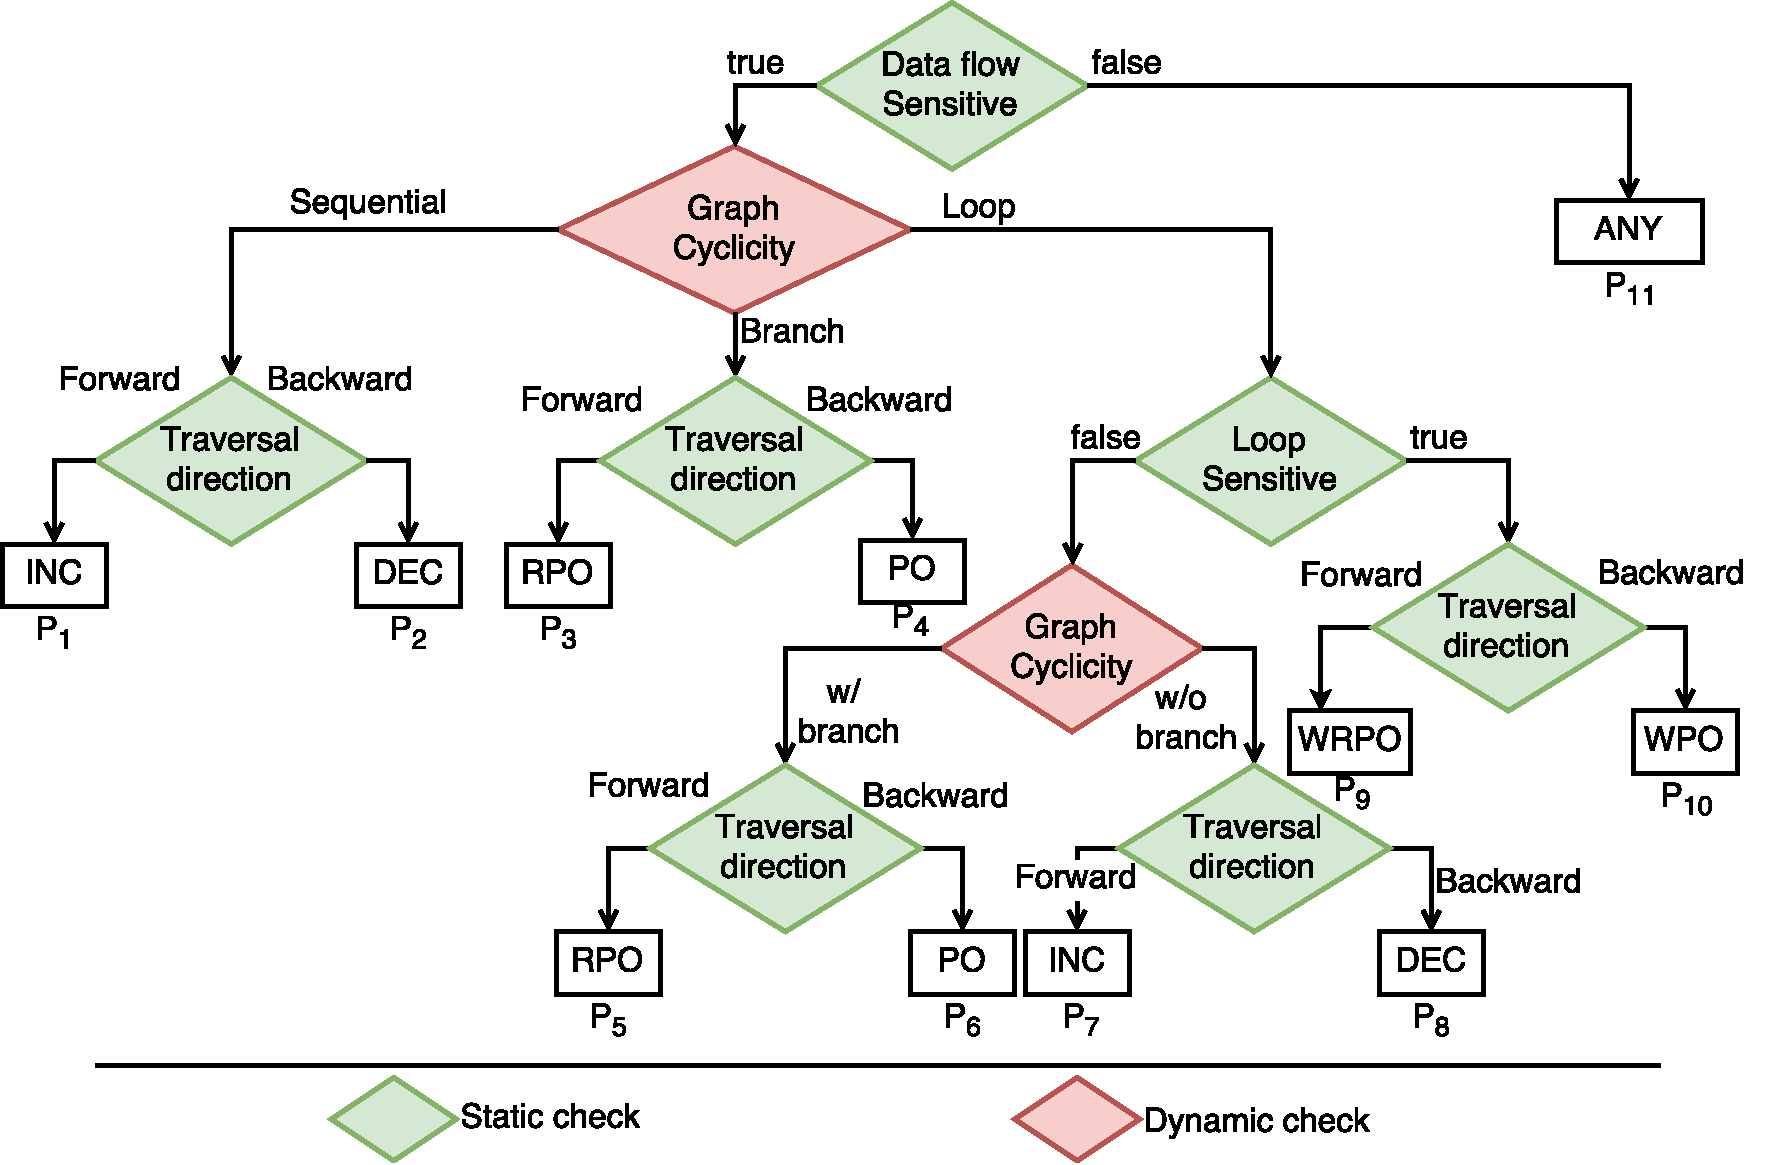
\includegraphics[width=0.8\linewidth]{figures/decision.pdf}
\caption{Traversal strategy selection decision tree.}
\label{fig:decision-diagram}
\end{figure}

\section{Decision Tree for Traversal Strategy Selection}
\label{sec:decision-tree}
At this point, we know the factors that influence the traversal strategy
selection: the static properties of the analysis, and the runtime property of
the graph. Our goal is to check these properties in certain order to quickly
decide the best traversal strategy for a given analysis and a graph, such that
only relevant properties are checked and the overhead of static/runtime check is
minimized\footnote{Our evaluation shows that the overhead is less than 0.2\% 
of the total running time for a large dataset and less than 0.01\% for an ultra-large dataset.}.
To that end, we carefully devised a decision tree as shown in
\fignref{fig:decision-diagram} for traversal strategy selection.

%\fignref{fig:decision-diagram} shows our decision tree for traversal strategy selection. 
The leaf nodes of the tree are one of the seven traversal strategies
and non-leaf nodes are static/runtime checks. The decision tree has eleven paths
marked $P_1$ through $P_{11}$. Given a traversal and an input graph, one of the
eleven paths will be taken to decide the best traversal strategy. The longest
paths $P_5$, $P_6$, $P_7$, and $P_8$ requires five checks and the shortest path
$P_{11}$ requires only one check. The static checks are marked green and the
runtime checks are marked red. The static properties that are checked are:
data-flow sensitivity ($P_{DataFlow}$), loop sensitivity ($P_{Loop}$), and
traversal direction. The runtime property that is checked is the graph
\graphprop{}: sequential, branch, loop w/ branch, and loop w/o branch. We now
provide rationale for arranging the decision tree as shown in
\fignref{fig:decision-diagram}.

The first property that is checked is the data-flow sensitivity of the
traversal. This is a static property determined by analyzing the traversal that
indicates whether the traversal output of any node is dependent on the traversal
output of its neighbors (successors or predecessors). This property is defined
in \defref{def:dataflow} and an algorithm to compute this property is given in
\algoref{algo:flow-sensitive}. The rationale for checking this property first is
that, if a traversal is data-flow insensitive ($P_{DataFlow}$ is
\textit{false}), irrespective of the type of the input graph, the traversal
can finish in a single iteration (no fixpoint computation is necessary). In
such cases, visiting nodes in any order will be efficient, hence we assign
any order (\textit{ANY}) traversal strategy (path $P_{11}$).

For traversals that are data-flow sensitive ($P_{DataFlow}$ is \textit{true}),
further checks are performed to determine the best traversal strategy. Next
property that is checked is the input graph \graphprop{}.
This is because the loop sensitive property is applicable to only graphs with
loops. 
\begin{itemize}
  \item \textit{Sequential Graphs (paths $P_1$ and $P_2$)}:
  In this type of graphs, no branches or loops exists, and all nodes have
  a single successor and predecessor.
  At this point, we know that the traversal is data-flow sensitive and it
  requires output of the neighbors to compute the output for any node. As
  sequential graphs have only one neighbor (successor or predecessor), a
  traversal strategy that visits the neighbor prior to visiting any node is
  sufficient to produce an optimal traversal order. To determine which neighbor
  (successor or predecessor), we check the traversal direction property. For
  \lstinline|FORWARD| traversal direction, predecessor of the node must be
  visited before the node and for \lstinline|BACKWARD| traversal direction,
  successor of the node must be visited before the node. These two traversal
  orders are provided by our \textit{INC} and \textit{DEC} traversal
  strategies. The corresponding paths in the decision tree are: $P_1$ and $P_2$.
  \item \textit{Graphs with branches (paths $P_3$ and $P_4$)}:
  In this type of graphs, branches exists, however loops don't exists, which
  means that a node may have more than one successor or predecessor. At this
  point, we know that our traversal is data-flow sensitive and it requires
  output of all neighbors (successors or predecessors) to compute the output for
  any node, we need a traversal order that ensures that all successors and
  predecessors are visited prior to visiting any node. This traversal order is
  given by the post-order (\textit{PO}) and reverse post-order (\textit{RPO})
  traversal strategies. To pick between \textit{PO} and \textit{RPO}, we check
  the traversal direction.
  For \lstinline|FORWARD| traversal direction, we need to visit all predecessors
  of any node prior to visiting the node, hence we pick the \textit{RPO}
  traversal strategy. For \lstinline|BACKWARD| traversal direction, we need to
  visit all successors of any node prior to visiting the node, hence we pick the
  \textit{PO} traversal strategy.
  \item \textit{Graphs with loops (paths $P_5$ to $P_{10}$)}: In this type of
  graphs, loops exists and in addition branches may also exists. We first need
  to check if the traversal is sensitive to the loop (the loop sensitive
  property). At this point, we know that our analysis is data-flow sensitive and
  the input graph has loop based control flow.
  	\begin{itemize}
	\item \textit{Loop sensitive (paths $P_9$ and $P_{10}$)}: When the traversal is
	loop sensitive, for correctly propagating the output, the traversal visits
	nodes multiple times until a fix point condition is satisfied (user may
	provide a fix point function). No iterative traversal strategy can guarantee
	that fix point will be reached in a single traversal of the nodes, hence we
	adopt a worklist based traversal strategy that visits only required 
	nodes (property of the worklist strategy). The worklist traversal strategy
	requires that the worklist (a data structure) is initialized with nodes.
	For picking the best order of nodes for initialization, we further investigate
	the traversal direction. We know that, for \lstinline|FORWARD| traversal
	direction, \textit{RPO} traversal strategy gives the best order of nodes and for
	\lstinline|BACKWARD| traversal direction, \textit{PO} traversal strategy gives
	the best order of nodes, we pick worklist strategy with reverse post-order
	\textit{WRPO} for \lstinline|FORWARD| and worklist strategy with post-order
	\textit{WPO} for \lstinline|BACKWARD| traversal directions.
	 \item \textit{Loop insensitive (paths $P_5$ to $P_8$)}: When the traversal is
	 loop insensitive, the selection problem reduces to the sequential and branch case
	 that is discussed previously, because for loop insensitive traversal, the
	 loops in the input graph is irrelevant and what remains relevant
	 is the existence of the branches.
  	\end{itemize}
\end{itemize}

\subsection{An Example}
\label{subsec:example}
In this section we explain the decision tree using an example source code analysis
and a graph.
The example analysis that we choose is the {\em Post Dominator Analysis} shown
in Listing \ref{lst:dominators} and the graph that we choose is shown in
\fignref{fig:running-example}.
The \textit{Post Dominator Analysis} contains two traversals: \lstinline|initT|
and \lstinline|domT|. 
The \lstinline|initT| traversal is data-flow insensitive ($P_{DataFlow}$ is
\textit{false}) and loop insensitive ($P_{Loop}$ is \textit{false}). The
\lstinline|domT| traversal is data-flow sensitive ($P_{DataFlow}$ is
\textit{true}) and loop insensitive ($P_{Loop}$ is \textit{false}). The
traversal directions of \lstinline|initT| and \lstinline|domT| are
\lstinline|ITERATIVE| and \lstinline|BACKWARD| respectively. 
Our example graph shown in \fignref{fig:running-example} has branches and loops, 
meaning the graph has nodes with more than one successor or
predecessor and has cycles.
% 
% 
% For \lstinline|initT| traversal, $P_{DataFlow}$ is
% \textit{false} and $P_{Loop}$ is \textit{false}, and for \lstinline|domT|
% traversal, $P_{DataFlow}$ is \textit{true} and $P_{Loop}$ is \textit{false}. The
% traversal directions of \lstinline|initT| and \lstinline|domT| traversals are
% \lstinline|ITERATIVE| and \lstinline|BACKWARD| respectively. The connectivity of
% input graphs can be anything in the set \{sequential, branch only, loop w/o
% branch, loop w/ branch\}. We now select an optimal traversal strategy for each
% of them.

For selecting the best traversal strategies for \lstinline|initT| and the graph
with loops and branches, we check the data-flow sensitivity property of the
traversal.
As \lstinline|initT| is data-flow insensitive, \textit{ANY} traversal strategy
is picked as shown by the path $P_{11}$ in \fignref{fig:decision-diagram} and no
further checks are required. The traversal strategy \textit{ANY} represents
nodes visited in any order.

For selecting the best traversal strategies for \lstinline|domT| and the graph
with branch and loop, we check the data-flow sensitivity property of the
traversal.
As \lstinline|domT| is data-flow sensitive, the next property to be checked is
the graph \graphprop{}. As our input graph has loops, the next property to be
checked is whether \lstinline|domT| is loop sensitive ie sensitive to the loops
present in the graph. Since \lstinline|domT| is loop-insensitive, we ignore the
loops present in the graph and investigate the rest of the graph structure. As
our graph contains branches, the next property to be checked is the traversal
direction. The traversal direction for \lstinline|domT| is \lstinline|BACKWARD|,
we pick \textit{PO} traversal strategy for \lstinline|domT| traversal, as shown
by the path $P_6$ in \fignref{fig:decision-diagram}. The traversal strategy
post-order (\textit{PO}) visits all successors of a node before visiting that
node. This is most suitable for backward analysis like \lstinline|domT|, because
backward analysis analyzes successors of a node prior to analyzing the node.

\section{Optimizing the Selected Traversal Strategy}
\label{subsec:optimizations}
The properties of the analysis and the input graph not only helps us select the
best traversal strategy, it also helps to perform several optimizations to the
selected traversal strategies. 

Running an analysis on a cyclic graph may require multiple iterations of the
nodes to compute the fixpoint solution. At least one additional traversal of the
nodes is required before the fixpoint check that compares the result of the last
two traversals to to ensure that results at nodes have stabilized. This
additional traversal and the fixpoint checks at nodes can be eliminated based on
the selected traversal strategy.

For data-flow insensitive traversals, we know that the traversal outputs of
nodes does not depend on the outputs of other nodes, hence both the additional
traversal and the fixpoint checks can be eliminated irrespective of the graph
cyclicity (path $P_{11}$ in our decision diagram
\fignref{fig:decision-diagram}).
In case of data-flow sensitive traversals, the traversal output of a node is
computed using the traversal outputs of other nodes (predecessors or
successors). For data-flow sensitive analysis on a acyclic graph provides an
opportunity to eliminate the additional traversal and fixpoint checks iff the
selected traversal strategy guarantees that the nodes whose outputs are required
to compute the output of a node are visited prior to visiting the node (paths
$P_1$ to $P_4$). 
In case of data-flow traversals, but loop insensitive traversals, and acyclic
graphs, the additional traversal and fixpoint checks can be eliminated iff the
selected traversal strategy guarantees that the nodes whose outputs are required
to compute the output of a node are visited prior to visiting the node (paths
$P_5$ to $P_8$).
The optimizations does not apply for traversals that are both data-flow and loop
sensitive, and the graph has cycles (paths $P_9$ and $P_{10}$). For such
traversals, our technique selects the worklist-based traversal strategy which
must perform fixpoint checks every time a node is visited.
% 
% 
% \begin{itemize}
%   \item {\em [\lstinline|Opt1|] Eliminating the result re-computation
%   traversal}:
%   A traversal that re-computes the results at graph nodes for enabling a fixpoint
%   traversal to compare the two results (the analysis traversal result and the
%   re-computation result) can be eliminated, if it is known that results have
%   stabilized and not going to change.
%   \item {\em [\lstinline|Opt2|] Eliminating the fixpoint check traversal}: If we know that the results have stabilized and eliminated the result re-computation traversal as a result, then the fixpoint check traversal is automatically eliminated as there is no result to compare the analysis traversal result.
% \end{itemize}
% 
% The same static and runtime checks that are performed to determine a traversal
% strategies also helps to determine if the optimizations can be performed. For
% instance, consider path $P_1$ in our decision tree shown in
% \fignref{fig:decision-diagram}. This path selects \textit{INC} traversal
% strategy that visits nodes in the increasing order of the node ids. While
% selecting this strategy, we came to know that the analysis is data-flow
% sensitive (which means the analysis output of neighbors (predecessors or
% successors) is required for computing the output of a node), the graph is
% sequential, (which means there is only one successor or predecessor), and the
% analysis is a forward analysis (which means the output of the predecessor is
% required to compute the output of a node). Together, we know that if a traversal
% strategy ensures that the predecessor is visited before visiting any node, the
% analysis output can be computed in one traversal and no fixpoint check is
% necessary. The traversal strategy selected for this path is \textit{INC} and it
% ensures this property. Hence, both \lstinline|Opt1| and \lstinline|Opt2| can be
% applied to the selected traversal strategy to further improve the performance.
% As we show in our evaluation (\secnref{sec:analysis-traversal-opt}), upto 60\%
% of the analysis time can be saved by performing these optimizations.
% 
% In our decision tree shown in \fignref{fig:decision-diagram}, all paths from
% $P_1$ to $P_8$ are eligible for both the optimizations. The paths $P_9$ and
% $P_{10}$ uses a worklist-based traversal strategy that visits only relevant
% nodes (relevant nodes are the nodes whose outputs have changed from the last visit)
% and must perform a fixpoint check every time a node is visited, hence the
% optimizations cannot be performed. Finally, for path $P_{11}$, the optimizations
% are not applicable, because data-flow insensitive traversals requires only
% one traversal to compute the results and no fixpoint check is performed. 
% 
% 
% , as data-flow insensitive analysis are single iteration
% analysis and hence the number of iterations cannot be reduced (\lstinline|Opt1|)
% and it does not involve fixpoint (\lstinline|Opt2|).
% The decision procedure begins by checking the data flow sensitivity property of
% the traversal ($P_{DataFlow}$). For \lstinline|initT| traversal, $P_{DataFlow}$
% is \textit{false}, hence \textit{SEQ} traversal strategy is picked as shown in
% \fignref{fig:decision-diagram} and no further checking is required. The
% traversal strategy \textit{SEQ} represents sequential order that visits nodes in
% the order they appear in the nodes list.
% For \lstinline|domT| traversal, $P_{DataFlow}$ is \textit{true}. The next static
% propery to be checked is loop sensitivity property ($P_{Loop}$), however
% $P_{Loop}$ is only applicable to graphs with loops, we check the connectivity
% property of the input graph.
% \begin{itemize}
%   \item For graphs with sequential connectivity, we check the traversal
%   direction and assign \textit{DEC} strategy (path $P_2$ in
%   \fignref{fig:decision-diagram}). This is because, for sequential graphs, the
%   traversal is expected to visit every node only once and visiting the nodes in
%   the decreasing order of the node ids ensures that the graph is visited in
%   the reverse order it was constructed. For instance, for visiting CFGs, the
%   decreasing order of the node ids gives the reverse control flow order of
%   nodes.
%   The \textit{DEC} traversal strategy benefits traversals that have backward
%   traversal direction. The \lstinline|domT| traversal is a backward traversal.
%   \item For graphs with branch connectivity, \textit{PO} is
%   picked for backward traversals (path $P_4$). This is because, in backward
%   traversals, outputs of successors is required for computing the output at
%   any node, and post order (\textit{PO}) visits all successors
%   of a node before visiting that node, hence \textit{PO} is picked.
%   \item For graphs with loop connectivity, loop sensitivity property
%   ($P_{Loop}$) is checked. For \lstinline|domT| traversal, $P_{Loop}$ is
%   \textit{false}. The next property to be checked is whether the graph also
%   contains branches along with loop. This is because, for loop insensitive
%   traversals, the loops in the input graph have no effect on the traversal order
%   and the selection decision reduces to with or without branches. For graphs
%   with branches, \textit{PO} is picked (path $P_6$), and for graphs without
%   branches, \textit{DEC} is picked (path $P_8$). The reasoning is similar to the
%   sequential and branch case described above.
% \end{itemize}

% To summarize, for \lstinline|initT| traversal, \textit{SEQ} traversal strategy
% is picked (path $P_{11}$ in our decision tree shown in
% \fignref{fig:decision-diagram}) and for \lstinline|domT| traversal, any of the
% following strategies can be picked based on the graph connectivity:
% \{\textit{DEC}, \textit{PO}\} (along paths $P_2$, $P_4$, $P_6$, $P_8$).
% Further, our hybrid checking enables applying optimizations to the selected
% traversal strategy. One such optimization is eliminating the fix point check for
% graphs that are sequential. The fix point checking requires an additional
% traversal of the graph, and for sequential graphs, the fix point check is not
% needed, as the traversal only requires one iteration.

% \section{Selecting and Optimizing the Traversal Order}
% \label{sec:select-optimize}
% 
% We model the selection of optimal traversal strategy using the decision tree
% shown in \fignref{fig:decision-diagram}. Inputs to our decision tree are: a
% traversal and a graph, and output is a traversal strategy selected from a list
% of candidate traversal strategies shown in \tabref{tab:strategies}.
% The decision tree checks both static properties about the traversal, and the
% dynamic properties about the input graph~\footnote{Note that, when we say
% dynamic properties about the input graph, we mean the connectivity of nodes in
% the graph, which is available only at runtime}.
% The static properties includes: data flow sensitivity, loop sensitivity, and
% traversal direction. The dynamic property is the graph connectivity that
% describes how nodes are connected to each others.
% Based on connectivity, we classified graphs into: \{sequential, branch only,
% loop w/o branch, loop w/ branch\}~\footnote{In case of sequential graphs, all
% nodes in the graph have no more than one successor and predecessor. In case of graphs
% with branches, nodes may have more than one successor or predecessor. In case of
% graphs with loops, there exists cycles in the graph.}.

% Here, we briefly describe the traversal strategy selection steps using the
% \textit{Post Dominator Analysis} given in Listing \ref{lst:dominators}, for
% input graphs with different connectivity.
% The \textit{Post Dominator Analysis} contains two traversals:
% \lstinline|initT| and \lstinline|domT|.
% For \lstinline|initT| traversal, $P_{DataFlow}$ is \textit{false} and $P_{Loop}$
% is \textit{false}, and for \lstinline|domT| traversal, $P_{DataFlow}$ is
% \textit{true} and $P_{Loop}$ is \textit{false}. The traversal directions of
% \lstinline|initT| and \lstinline|domT| traversals are \lstinline|ITERATIVE| and
% \lstinline|BACKWARD| respectively.
% The connectivity of input graphs can be anything in the set \{sequential, branch
% only, loop w/o branch, loop w/ branch\}.
% We now select an optimal traversal strategy for each of them.

% The decision procedure begins by checking the data flow sensitivity property of
% the traversal ($P_{DataFlow}$). For \lstinline|initT| traversal, $P_{DataFlow}$
% is \textit{false}, hence \textit{SEQ} traversal strategy is picked as shown in
% \fignref{fig:decision-diagram} and no further checking is required. The
% traversal strategy \textit{SEQ} represents sequential order that visits nodes in
% the order they appear in the nodes list.
% For \lstinline|domT| traversal, $P_{DataFlow}$ is \textit{true}. The next static
% propery to be checked is loop sensitivity property ($P_{Loop}$), however
% $P_{Loop}$ is only applicable to graphs with loops, we check the connectivity
% property of the input graph.
% \begin{itemize}
%   \item For graphs with sequential connectivity, we check the traversal
%   direction and assign \textit{DEC} strategy (path $P_2$ in
%   \fignref{fig:decision-diagram}). This is because, for sequential graphs, the
%   traversal is expected to visit every node only once and visiting the nodes in
%   the decreasing order of the node ids ensures that the graph is visited in
%   the reverse order it was constructed. For instance, for visiting CFGs, the
%   decreasing order of the node ids gives the reverse control flow order of
%   nodes.
%   The \textit{DEC} traversal strategy benefits traversals that have backward
%   traversal direction. The \lstinline|domT| traversal is a backward traversal.
%   \item For graphs with branch connectivity, \textit{PO} is
%   picked for backward traversals (path $P_4$). This is because, in backward
%   traversals, outputs of successors is required for computing the output at
%   any node, and post order (\textit{PO}) visits all successors
%   of a node before visiting that node, hence \textit{PO} is picked.
%   \item For graphs with loop connectivity, loop sensitivity property
%   ($P_{Loop}$) is checked. For \lstinline|domT| traversal, $P_{Loop}$ is
%   \textit{false}. The next property to be checked is whether the graph also
%   contains branches along with loop. This is because, for loop insensitive
%   traversals, the loops in the input graph have no effect on the traversal order
%   and the selection decision reduces to with or without branches. For graphs
%   with branches, \textit{PO} is picked (path $P_6$), and for graphs without
%   branches, \textit{DEC} is picked (path $P_8$). The reasoning is similar to the
%   sequential and branch case described above.
% \end{itemize}
% 
% To summarize, for \lstinline|initT| traversal, \textit{SEQ} traversal strategy
% is picked (path $P_{11}$ in our decision tree shown in
% \fignref{fig:decision-diagram}) and for \lstinline|domT| traversal, any of the
% following strategies can be picked based on the graph connectivity:
% \{\textit{DEC}, \textit{PO}\} (along paths $P_2$, $P_4$, $P_6$, $P_8$).
% Further, our hybrid checking enables applying optimizations to the selected
% traversal strategy. One such optimization is eliminating the fix point check for
% graphs that are sequential. The fix point checking requires an additional
% traversal of the graph, and for sequential graphs, the fix point check is not
% needed, as the traversal only requires one iteration.



% 
% 
% For instance, for CFGs, if there exists conditional branch instructions,
% such as \lstinline|if|, \lstinline|switch|, etc, the branch control flow
% property set to \textit{true}. If there exists loop instructions, such as
% \lstinline|for|, \lstinline|while|, etc, the loop based control flow property is
% set to \textit{true}. Based on branch control flow property and loop based
% control flow property, every CFG is assigned one of the below four control flow
% property:
% \begin{itemize}
%   \item sequential control flow
%   \item branch control flow
%   \item loop w/ branch control flow
%   \item loop w/o branch control flow
% \end{itemize}
